% \chapter*{Abstract}

% Apparently the GOST for dissertations does not include an abstract

\addcontentsline{toc}{chapter}{Introduction}
\chapter*{Introduction}

% Template and formatting:
% All Skoltech theses have an abstract
% One thesis had chapter summary at the end of each chapter. Looks like a good idea
% Introduction is apparently just a regular chapter


\subsection*{Relevance of the work} 

This work considers the quantum model of computation. In this model, classical bits -- modelled by Boolean variables -- are replaced by qubits, modelled by two-dimensional complex vector spaces. The key effects enabling the quantum computations are quantum superposition and quantum entanglement. While the state space of $n$ bits is a Cartesian product of individual state spaces, the state space of $n$ qubits is the \textit{tensor} product of individual spaces. Because of this, a state of the qubits can in principle be not factorizable into single-qubit states. This, on the one hand, enables quantum computers to process many different classical bit states in parallel, and on the other hand, makes them extremely difficult to simulate by classical means: naively simulating a quantum device with $n$ qubits requires working with $2^n$-dimensional complex vectors.

The complexity class of problems efficiently solved by a quantum computer is called $\mathbf{BQP}$. While it is not known how $\mathbf{BQP}$ relates to $\mathbf{P}$, the class of problems efficiently solved by a classical computer, the former contains problems that do not yet have an efficient classical solutions. The most famous example of that was found with the discovery of Shor's algorithm, which enables quick factorization of integer numbers in their prime factors and, consequently, the defeat of hitherto unbreakable algorithms of encryption \cite{nielsen_quantum_2010}.

The appeal of quantum computers is offset by the notorious difficulty of making them in practice. While the current devices are far more advanced than the first proof-of-concept devices, they are still a long way from the characteristics that would enable them to, e.g.,~run the Shor's algorithm for any practical means. 
The limitations of physical quantum computers come from extreme fragility of quantum states. The quantum logic gates are not performed with perfect accuracy, the qubits themselves lose coherence over time, and there is even a probability of incorrect measurement, meaning that even the correct quantum state can be read with errors. For this reason, the current generation of quantum computers is referred to as noisy intermediate-scale quantum (NISQ) devices \cite{bharti_noisy_2021}.

While large-scale, fault-tolerant quantum computers are a long way ahead, there is research effort towards developing algorithms that can work within the limitations of NISQ devices. One such family of quantum algorithms is called variational quantum algorithms \cite{cerezo_variational_2020}. Such algorithms are designed to solve optimization problems. The broad idea of these algorithms is to encode the solution to the problem in a parametrized quantum state (called an ansatz), so that a series of measurements on that state can give an estimate of the cost function to be minimized. Then the parameters of the state are tuned so as to deliver a minimum to the cost function. The range of problems that can be addressed by this approach is rather extensive: from classical optimization problems, like the travelling salesepson problem, to problems that arise in quantum chemistry and quantum physics, e.g.~investigation of the potential landscape of chemical reactions~\cite{reiher_elucidating_2017} and ground state properties of electronic lattices~\cite{cade_strategies_2019}. Another important branch of study is devoted to quantum machine learning with variational algotihms~\cite{skolik_layerwise_2020,havlicek_supervised_2019,schuld_circuit-centric_2020}. In that approach, a quantum device acts as a classifier that is trained to partition data points encoded as quantum states.

(a paragraph about vqe here?)

Despite the simplicity of the approach, the variational quantum algorithms are far from being understood well. Since they involve optimization, there are lots of questions concerning the convergence of this optimization, the properties of the cost function landscape, the choice of the circuits, etc. This dissertation contributes to the literature both in numerical experiments and in theoretical results.

\subsection*{Dissertation goals} 

The goal of this dissertation is to investigate the performance of variational quantum algorithms and to further the theoretical understanding of their behavior. To achieve this goal, we set up and performed the following tasks:

\begin{enumerate}
    \item Develop a numerical implementation the variational quantum eigensolver algorithm and study its convergence for physical problems. Study its dependence on the depth of the circuit, number of qubits, and other relevant parameters.
    \item Develop a numerical implementation of a quantum classifier and investigate its properties. In particular, study its ability to learn on quantum data, namely on quantum states obtained using VQE.
    \item Study the physically relevant properties of the VQE-optimized solutions for the next-nearest-neighbor Hubbard model. Analyze the behavior of gradients in the associated optimization problem.
    \item Calculate a bound on the variance of derivatives of Hamiltonian cost functions with respect to random selection of circuit parameters. Estimate the onset of the barren plateau regime with the increasing depth and connectivity of a parametrized quantum circuit.
    \item Develop an algorithm for bounding the fidelity of the Greenberger-Horne-Zeilinger state and other Clifford states based on their parent Hamiltonian.
\end{enumerate}

\subsection*{Statements defended}

\begin{enumerate}

    \item We applied Adiabatically-assisted VQE (AAVQE) to the ground state problem for the Heisenberg XXZ model, i.e.~the family of spin Hamiltonians of the type 
    \begin{equation*}
        H(h) = \sum_{i=1}^{n} X_i X_{i+1} + Y_i Y_{i+1}+ h Z_i Z_{i+1},
    \end{equation*}
    where $X_i, Y_i$, and $Z_i$ are respective Pauli matrices acting on $i$'th spin. AAVQE consists in using the solution for $H(h)$ as a starting point of the optimization process for $H(h + \delta h)$, eventually finding an approximate ground state for a range of parameters $[h_{\mathrm{min}}, h_{\mathrm{max}}]$. Numerical experiments show that Adiabatically-assisted VQE finds different solutions depending on the direction of whether the optimization starts from $h_{\mathrm{min}}$ and increases $h$, or starts from $h_{\mathrm{max}}$ and gradually decreases $h$. Specifically, the largest difference occures near the critical point of the model ($h = 1$). In contrast, the transverse-field Ising model shows no such behavior near the critical point: both methods of running AAVQE yield the same ground state energies up to the tolerance of the optimizer.
    \item The approximation found by VQE shows the largest energy error in the vicinity of the critical point of either spin model. For the best ans\"atze considered, the maximum energy error is $0.12$ units for the Ising model and $1.1$ units for the Heisenberg model. We argue that this is consistent with the fact that critical states demonstrate a logarithmic scaling of entanglement entropy, 
    unattainable by a fixed-depth ansatz circuit.
    \item We proposed a quantum classifier which demonstrates that quantum machine learning models can partition quantum data. The classifier was tested for ten qubits on the VQE-approximated ground states of transverse-field Ising model and was able to predict the phase of the system with 97\% accuracy. A similar experiment conducted for the Heisenberg XXZ model yielded 93\% accuracy.

    \item Variational quantum eigensolver was numerically applied to a Hubbard-like model, with ansatz depth ranging from one to ten layers. For 4 qubits and fewer, VQE found the exact solution up to machine precision with 1-2 layers. For 5-11 qubits, the error scaling with depth was fit to exponential decay (correlation coefficient between depth and $\log_{10} \Delta E$ was $-0.92$ or less in all cases).
    
    \item We estimated the variance of partial derivatives of the energy cost function for the next-nearest-neighbor Hubbard model in 4-10 qubits by random sampling of the ansatz parameters. The model was transformed to a qubit Hamiltonian by Jordan--Wigner and Bravyi--Kitaev transformations. 
    We observed that, under the Jordan--Wigner transformation, the dependence of the variance on circuit depth becomes constant after at most 15 layers. The behavior of the variance as a function of the number of qubits is consistent with the prediction of exponential decay given in \cite{mcclean_barren_2018}.
    For the Bravyi--Kitaev transform we observed a longer transient behavior with the circuit depth.
    \item We derived a lower bound on the variance of derivatives for parametrized quantum circuits composed of blocks that constitute local 2-designs. Let the block that depends on a real parameter $\theta$ be situated in layer $l_c$ out of $l$ layers total. Then the variance $\Var \partial_\theta E$ behaves as
    \begin{equation*}
        \Var \partial_\theta E \in \sum_h \Omega\left(3^{-|C(h)|} \left(\frac{3}{4}\right)^{l-l_c}\right).
    \end{equation*}
    Here the sum is taken over every Pauli string $h$ in the Pauli decomposition of the cost function, and $|C(h)|$ is the size of the causal cone of this Pauli string.
    \item We developed an algorithm to estimate the fidelity of Clifford states using at most $n$ series of Pauli measurements, where $n$ is the number of qubits. 
\end{enumerate}

\subsection*{Scientific novelty}
% It seems that statements to defend can very much overlap with the sci novelty, at least in some examples they do.
\begin{enumerate}
    \item In the original proposal \cite{garcia-saez_addressing_2018}, the adiabatically-assisted VQE algorithm was used for a family of Hamiltonians $H(\tau)$ such that $H(0)$ is an easily-solved problem, while $H(1)$ encodes a difficult problem. For the transverse-field Ising and Heisenberg models, the ground state problem dependence on the parameter can be characterized as <<easy, hard, easy>>: $H(0)$ is easy to solve, $H(1)$ is difficult, then in the limit of $\tau \rightarrow \infty$ the problem $H(\tau)$ again becomes easy.
    \item We demonstrated that a quantum classifier can be trained on intrinsically quantum data. Prior art appears to focus on classification problems based on classical input data.    
    \item For fermionic Hamiltonians, the onset of barren plateaus phenomenon was shown to occur differently depending on the choice of fermion-to-qubit mapping, which was previously not considered in the literature.
    \item We derived a lower bound on the variance of the derivatives of cost function with respect to ansatz parameters. Compared to the existing literature \cite{mcclean_barren_2018,cerezo_cost-function-dependent_2020}, our estimate depends only on the size of the causal cone of the circuit and is applicable to quantum circuits of arbitrary topology (as long as they consist of two-qubit blocks that constitute approximate 2-designs).
    % we applied the theory of $t$-designs in the Heisenberg picture, considering the random unitaries as operators acting on Pauli strings of $2n$ qubits (which we dubbed super Pauli strings).
    \item We proposed a method of estimating fidelity for the GHZ state that only involves two series of measurements. The method relies on the relation between the energy of a state with respect to a Hamiltonian and the fidelity between that state and the ground state (the stability lemma).
\end{enumerate}

\subsection*{Theoretical and practical significance} Classification of quantum phases by quantum means is potentially useful for condensed matter physics. The results on the convergence of VQE are important for the design of quantum optimization algorithms. The proposed method for validating the GHZ state is potentially useful for evaluating the properties of quantum devices in a simple manner.
Practical significance of the work is supported by the usage of the results in delivering the RFBR grant No.\ 19-31-90159 ``Aspiranty''.

The \textbf{validity of the work} is supported by numerical experiments and rigorous mathematical proofs, where applicable.

\subsection*{Presentations and validation of the results}
The main results of the work have been reported in the following scientific conferences and workshops:

\begin{enumerate}
    \item International Conference on Quantum Technologies (July 15-19, 2019, Moscow, poster);
    \item 62nd MIPT conference (Nov 18-24, 2019, Moscow, talk);
    \item Inaugural Symposium for Computational Materials Program of Excellence (September 4-6, 2019, Moscow, poster);
    \item International School on Quantum Technologies (March 1-7, 2020, Sochi, poster);
    \item International Conference on Quantum Technologies (July 12-16, 2021, Moscow, online, poster);
    \item QuOne workshop on Quantum Machine Learning (Feb 22-24, 2022, Tehran, online, talk).
\end{enumerate}

\subsection*{Structure of the dissertation} The dissertation consists of introduction, six chapters, conclusions, bibliography, list of symbols and abbreviations, list of tables, list of figures, and supplemental material.

\subsection*{Publications}
The work in this thesis is based on the following publications:

\begin{enumerate}
    \item \fullcite{uvarov_machine_2020}
    \item \fullcite{uvarov_variational_2020}
    \item \fullcite{uvarov_barren_2021}
\end{enumerate}

\subsection*{Acknowledgments} I thank my advisor, Jacob Biamonte, for providing guidance and assistance at all stages of my doctoral study. I also thank my coauthors, Dmitry Yudin and Andrey Kardashin for a productive collaboration. I am grateful to Akshay Vishwanathan, Richik Sengupta, Soumik Adhikary, Daniil Rabinovich, Hariphan Philathong, Oksana Borzenkova, Ernesto Campos, Aly Nasrallah, and Mauro Morales for numerous insightful discussions. Last but not least, I thank my family and my friends for immense support during my scientific journey.

\chapter{Main concepts in quantum computation}
\label{chap:quantum_basics}

In this chapter, we will briefly review the basic mathematical concepts necessary to reason about quantum computers. For a more extensive introduction, we refer the reader to the classic textbooks: \cite{nielsen_quantum_2010,kitaev_classical_2002}.

\section{Definitions and notation}

A \textit{qubit} is a quantum system with two controllable states. We will model such a system with a two-dimensional state space $\mathbb{C}^2$ with a distinguished orthonormal basis, called the \textit{computational basis} and denoted as $\{ \ket{0}, \ket{1} \}$. The Hilbert space\footnote{Throughout the thesis, we will only work in finite-dimensional Hilbert spaces.} $\mathcal{H}$ of $n$ qubits is the complex vector space $(\mathbb{C}^2)^{\otimes n}$. \textit{Pure states} of the qubits are the vectors $|\psi \rangle \in \mathcal{H}$ of norm one. 
% Generic quantum states are described as positive semidefinite (or nonnegative) operators on $\mathcal{H}$ called \textit{density operators}, \textit{density matrices}, or \textit{mixed states} (more on that later). The former can be included in the latter: a projector $\ket{\psi} \bra{\psi}$ is a bona fide density operator.

The standard basis for the registry of $n$ qubits, also called the computational basis, is the tensor product of individual computational bases. 
When writing such basis states, we will omit the tensor product: for example, $\ket{0} \otimes \ket{0} \otimes \ket{1} \equiv \ket{001}$.

A key feature of quantum states is entanglement:

\begin{definition}
    A state $\ket{\psi} \in \mathcal{H}_1 \otimes \mathcal{H}_2$ is \textit{entangled} if there are no states $\ket{\phi_1} \in \mathcal{H}_1, \ \ket{\phi_2} \in \mathcal{H}_2$ such that $\ket{\psi} = \ket{\phi_1} \otimes \ket{\phi_2}$. Otherwise, the state is called \textit{separable} with respect to the bipartition $\mathcal{H} = \mathcal{H}_1 \otimes \mathcal{H}_2$. If an $n$-qubit state can be presented as a tensor product of $n$ single-qubit states, it is called a \textit{separable} or a \textit{product state}.
\end{definition}

\begin{example}
    The \textit{Bell state} $\ket{\Phi} = \frac{1}{\sqrt{2}}(\ket{00} + \ket{11})$ is an example of an entangled state of two qubits. This is easy to check: an arbitrary separable state of two qubits has the form $(\alpha \ket{0} + \beta \ket{1}) \otimes (\gamma \ket{0} + \delta \ket{1})$. By comparing the coefficients, we arrive to the following system of equations that has no solutions:
    \begin{equation}
        \left\{
            \begin{array}{rl}
                \alpha \gamma = & \frac{1}{\sqrt{2}} \\
                \beta \delta = & \frac{1}{\sqrt{2}} \\
                \alpha \delta = & 0 \\
                \beta \gamma = & 0 \\
            \end{array}
        \right.     
    \end{equation}
    The $n$-qubit analog of the Bell state $\ket{\Psi} = \frac{1}{\sqrt{2}}(\ket{0...0} + \ket{1...1})$ is known as the \textit{Greenberger--Horne--Zeilinger state} or as the \textit{Schr\"odinger's cat state}.
\end{example}


The space of linear operators on $\mc{H}$ can be equipped with a Hilbert-Schmidt inner product:
\begin{equation}
(A, B) = \frac{1}{\mathrm{dim} \mc{H}} \Tr A^\dagger B.
\end{equation}
Relative to this inner product, the space of linear operators on $\mc{H}$ admits an orthogonal basis of \textit{Pauli strings}, which are tensor products of \textit{Pauli matrices}:

\begin{definition}[Pauli matrices]
    \textit{Pauli matrices} are the $2 \times 2$ identity matrix $\id$ and the following three $2 \times 2$ matrices:
    \begin{equation}
        X = \begin{pmatrix}
            0 & 1 \\ 1 & 0 
        \end{pmatrix}, \ 
        Y = \begin{pmatrix}
            0 & -\mathrm{i} \\ \mathrm{i} & 0 
        \end{pmatrix}, \ 
        Z = \begin{pmatrix}
            1 & 0 \\ 0 & -1
        \end{pmatrix}.
    \end{equation}
\end{definition}

\begin{definition}[Pauli string]
A \emph{Pauli string} is a tensor product of $n$ Pauli matrices $\{\id, X, Y, Z \}$. The $n$-qubit identity operator $\id \otimes \id \otimes ... \otimes \id$ is the \emph{trivial} or \textit{unit} string. The \textit{algebraic locality} or just \textit{locality} of a Pauli string is the number of non-identity Pauli matrices contained in the string.
% For qudits, one should instead use Gell-Mann matrices, but throughout the text we will nonetheless refer to that object as a Pauli string.
\end{definition}

Since the product of two Pauli strings is, up to a multiple of $\rmi$, a Pauli string, it is sometimes important to consider the \emph{Pauli group} consisting of all Pauli strings, possibly multiplied by $\rmi$, $-1$, or $-\rmi$.

The expansion of the operator in the basis of Pauli strings will be called its \textit{Pauli decomposition}. For a Hermitian operator $H$ on $\mc{H}$ in a given orthonormal basis, we will call its \textit{locality} $\operatorname{loc} H$ the maximum locality of its terms in the decomposition and its \textit{cardinality} $\operatorname{card} H$ the number of Pauli strings in the decomposition. Note that for a Hermitian operator, the coefficients of the Pauli decomposition will be real.

All Pauli strings have eigenvalues $\pm 1$. The eigenbases of individual Pauli matrices are also important. The computational basis is the eigenbasis for the $Z$ matrix. The eigenstates of the $X$ matrix are known as the plus state and the minus state: $\ket{+} = \frac{1}{\sqrt{2}}(\ket{0} + \ket{1}), \ \ket{-} = \frac{1}{\sqrt{2}}(\ket{0} - \ket{1})$. The eigenstates of $Y$ are $\ket{y_\pm} = \frac{1}{\sqrt{2}}(\ket{0} \pm \mathrm{i} \ket{1})$.

In the basis of Pauli strings, the Gram matrix of the Hilbert-Schmidt inner product is the identity matrix. In fact, $\operatorname{Herm}(2^n)$ behaves like $\mathbb{R}^{4^n}$ equipped with the standard inner product. Because of that, for an operator $A = \sum c_\alpha \sigma_\alpha$, written in its Pauli decomposition, we will occasionally be interested in $p$-norms of the vector of its coefficients $||\{c_\alpha\}||_p$.

\begin{proposition}
    \label{prop:ad_is_pauli_orthogonal}
    Let $U$ be a unitary operator on $\mc{H}$. Denote $\operatorname{Ad}_U$ the operator of conjugation by $U$: 
    \begin{align}
        \operatorname{Ad}_U: \operatorname{End}(\mc{H}) &\rightarrow  \operatorname{End}(\mc{H}) \\
        \operatorname{Ad}_U(X) &= U^\dagger X U
    \end{align}
    This operator is unitary on $\operatorname{End}(\mc{H})$ and orthogonal on $\operatorname{Herm}(\mc{H})$  (when the latter is considered as a real vector space spanned by Pauli strings).
\end{proposition}
\begin{proof}
    If $H$ is Hermitian, $U^\dagger HU$ is also Hermitian, so $\operatorname{Herm}(\mc{H})$ is an invariant subspace of $\operatorname{Ad}_U$. The Hilbert--Schmidt product $(A, B) = \Tr(A^\dagger B)$ is preserved under the conjugation of both factors: $\operatorname{Tr} (U^\dagger A^\dagger U U^\dagger B U) = \operatorname{Tr} (A^\dagger B)$.
\end{proof}

In particular, it follows that the vector 2-norm of a Hermitian operator (i.e.~the sum of the squares of its Pauli coefficients) is preserved under $\operatorname{Ad}_U$.

\section{Quantum model of computation}

% TODO needs examples of unitaries: rotations, Hadamard, CNOT, maybe MS

What operations can be performed on idealized qubits? The basic building blocks of any quantum algorithm are (i) quantum gates and (ii) measurements. 

\subsubsection{Quantum gates}

Quantum gates are represented by unitary matrices $UU^\dagger = \id$. We say that a quantum gate $U$ is an $m$-qubit gate if the gate is supported only on $m$ qubits. That is, there is a subset of $m$ qubits such that, under proper ordering of the tensor factors, $U$ can be represented as $V \otimes \id$ for some $V \in U(2^m)$.

A quantum computer is assumed to be able to produce few-qubit quantum gates from some fixed set. A sequence of quantum gates, together with measurements (see next paragraph) and possibly gates conditioned on classical measurements, is called a \textit{quantum circuit}. 

We highlight two key features of unitary maps:

\begin{enumerate}
    \item Unitary means reversible. We cannot erase information. Thus, we cannot naively implement quantum analogs of AND and OR gates. However, with some extra effort, classical logic gates can still be embedded in quantum gates.
    \item Multi-qubit gates can produce entanglement.
\end{enumerate}



Sometimes a quantum gate will depend on a real parameter. In this case, the circuit containing such gates will be called a \textit{parametrized quantum circuit}. We will assume that this dependence is infinitely differentiable. In the context of variational quantum algorithms, a parametrized quantum circuit is sometimes called an \textit{ansatz}.

\begin{example}
    A single-qubit rotation $R_Y(\theta) = e^{-\rmi Y \theta / 2}$ is a parametrized quantum gate. The fact that $Y^2 = \id$ enables the following decomposition: $R_Y(\theta) = \cos (\theta/2) \id - \rmi \sin (\theta / 2) Y$.
\end{example}

\subsubsection{Measurements}

In general, when we measure a quantum system, we measure some kind of \textit{observable}, i.e.~a Hermitian operator. Let $A$ be some observable with eigenvalues $\lambda_i$ and corresponding eigenstates $\ket{\lambda_i}$. Let the system be in the state $\ket{\psi} = \sum c_i \ket{\lambda_i}$. Then, upon measurement, we will observe the value $\lambda_i$ with probability $|c_i|^2$. The expected value of the measurement outcome is $\sum_i |c_i|^2 \lambda_i$. If the measurement does not destroy the system (e.g.~in photonic quantum computing, measuring a qubit effectively destroys it), the state after measurement with outcome $\lambda$ can be described by the following \textit{density operator} (see Section \ref{subsec:mixed}):
\begin{equation}
    \label{eq:postmeasurement}
    \rho_{\text{post}} = \frac{\Pi_\lambda \ket{\psi}\bra{\psi} \Pi_\lambda}{\Tr (\ket{\psi}\bra{\psi} \Pi_\lambda)},
\end{equation}
where $\Pi_\lambda$ is the projector on the eigenspace of $\lambda$. If the eigenspace is one-dimensional, the language of density operators can be avoided: in such case, the post-measurement state is a pure state $\ket{\psi}$.

Different observables can be measured simultaneously if and only if the corresponding operators have a shared eigenbasis. Sometimes we only care about the basis itself, so the observables we measure are projectors on the basis states: $P_1 = \ket{e_1} \bra{e_1}, ..., P_k = \ket{e_k} \bra{e_k}$. We then say that we measure in the basis $(e_1, ..., e_k)$.

Without any extra effort, a quantum computer makes a $Z$ measurement on each qubit. To measure qubits in different bases, one should apply single-qubit or multi-qubit unitaries before measurement. For example, if we want to measure the qubits in the $\{ \ket{+},\ket{-} \}$ basis, we should apply a Hadamard gate to the qubit. If we would like to measure the qubits in some entangled basis, we would have to apply some multi-qubit gates before the measurement. Since single-qubit operations are easier to perform than multi-qubit operations, we mostly consider measurements of observables that don't need entangled bases, such as Pauli strings.

\section{Noise and decoherence}

\subsection{Mixed states and density matrices}
\label{subsec:mixed}
By the very nature of quantum computation as external manipulation of the qubits, it is not enough to consider the qubits as isolated physical entities. In order to focus on the behavior of qubits, though, one can ``trace out'' the irrelevant degrees of freedom, while preserving their action on the qubits. To do that, we represent quantum states not as vectors in $\mc{H}$, but as a certain kind of linear operators on $\mc{H}$. A pure state $\ket{\psi} \in \mc{H}$ is mapped to an operator $\rho := \ket{\psi}\bra{\psi} \in \mathrm{End}(\mc{H})$. The expected value of an observable $B$ is now equal to $\Tr (\rho B)$.


Now, consider a state space of two subsystems $\mc{H} = \mc{H}_1 \otimes \mc{H}_2$. Denote $\{\ket{e_i}\}$ the basis of $\mc{H}_1$ and $\{\ket{f_j}\}$ the basis of $\mc{H}_2$. If we measure some observable $A$ only on the first subsystem, that is equivalent to measuring $A \otimes I$ on the entire system. If the state is equal to $\sum_{ij} c_{ij} \ket{e_i} \ket{f_j}$, then the density matrix is equal to $\sum_{ijkl} c^*_{ij} c_{kl}\ket{e_k} \ket{f_l}\bra{e_i} \bra{f_j}$. The expected value will now be equal to $\sum_{ijkl} c^*_{ij} c_{kl} A_{ik} \delta_{jl}$, which means that the only relevant information in $\rho$ is stored in its \textit{partial trace}:

\begin{equation}
    [\rho_{\mc{H}_1}]_{ik} := \sum_l \rho_{ilkl}.
\end{equation}

This partial trace now has a few remarkable properties:

\begin{enumerate}
    \item The operator $\rho_{\mc{H}_1}$ can be represented as $\ket{\phi}\bra{\phi}$ for some $\ket{\phi} \in \mc{H}_1$ if and only if the full state $\ket{\psi}$ is biseparable;
    \item the $i$'th diagonal entry of $\rho_{\mc{H}_1}$ contains the probabilities of observing the system in the state $\ket{e_i}$;
    \item the trace of $\rho_{\mc{H}_1}$ is equal to one as probabilities of all possible events sum up to one.
\end{enumerate}

Such operators are called \textit{density operators} or \textit{density matrices}. These operators are non-negative operators with trace equal to one. The space of density operators includes pure states as a subset, but it also brings new objects.

Any density matrix can be diagonalized (because any non-negative operator is also a Hermitian operator), i.e.~there is a basis $e_i$ such that

\begin{equation}
    \rho = \sum_i p_i \ket{e_i}\bra{e_i}.
\end{equation}

When such a diagonalization has only one term, we call $\rho$ a pure state, otherwise it is called a \textit{mixed state}. Note that the state is pure if and only if $\rho^2 = \rho$.

There are several metrics to estimate the mixedness of a state. The simplest one is \textit{purity}, which we define as $\Tr{\rho^2}$. The more complicated measure is the \textit{von Neumann entropy}:

\begin{equation}
    S(\rho) = - \Tr \rho \log \rho.
\end{equation}

This formula makes sense even when $\rho$ has zero eigenvalues because $\lim_{x \rightarrow 0^+} x \log x = 0$. The units of $S(\rho)$ are called \textit{nats} if the formula uses the natural logarithm, and \textit{bits} or \textit{ebits} if the logarithm is base two. 

The Bell state $\ket{\Phi} = \frac{1}{\sqrt{2}}(\ket{00} + \ket{11})$ has exactly one ebit of entropy: the reduced density matrix of any qubit is simply $\frac12 \id$, hence the entropy is equal to $-\log \frac{1}{2}$ nats or $-\log_2 \frac{1}{2} = 1$ ebit. For that reason, the states that are obtaied from the Bell state by application of local unitary operators are called \textit{maximally entangled states} in two qubits.

Unfortunately, estimating von Neumann entropy in practice is hard. An alternative measure, called $\alpha$-\textit{R\'enyi entropy}, is defined for $\alpha \geq 0, \alpha \neq 1$ as follows:

\begin{equation}
    S_\alpha (\rho) = \frac{\log \Tr \rho^\alpha}{1 - \alpha}.
\end{equation}

For $\alpha \rightarrow 1$, the limit of such entropy is the von Neumann entropy. For the 2-R\'enyi entropy, there is an efficient estimation protocol \cite{brydges_probing_2019}.

When we introduced the density matrix formalism, we assumed that there are two subsystems, and found that the reduced density matrix can provide information about the entanglement between the subsystems. However, this also works if one of the subsystem is the entire quantum registry, and the other subsystem is the rest of the Universe. Without going into the details of interpretations of quantum mechanics, we can say the ``entanglement with the Universe'' is practically observed as decoherence of the quantum system. For instance, a \textit{maximally mixed state} $\rho = \frac{1}{\operatorname{dim} \mc{H}} \id$ will return uniformly random measurement outcomes in any basis, meaning that a coherent quantum state is completely lost. In addition, a diagonal density matrix can describe a classical probability distribution, without any quantum correlations. For instance, if your experimental apparatus prepares a state $\ket{0}$ with probability $p$, and a state $\ket{1}$ with probability $1 - p$ (without telling you which is the case), then you can describe the state of your system with a density matrix equal to $\operatorname{diag}(p, 1- p)$.




% When considering pure states is not enough, we will work with states as positive semidefinite Hermitian operators $\rho \in \mathrm{End}(\mathcal{H})$, whose trace is equal to one. If the rank of $\rho$ is equal to one, the state is called a pure state, otherwise it is a \textit{mixed state}.



% Quantum mechanics has a way to describe such situations using the formalism of \textit{density matrices}. The states that are described this way are called \textit{mixed states}:

% \begin{definition}[mixed state]
%     adsf
% \end{definition}

% \begin{definition}[density matrix]
%     A density matrix on $\mathcal{H}$ is a positive semidefinite linear operator.
% \end{definition}


\subsection{Quantum channels}

For pure states, the only operations we could perform were the unitary maps. For density operators, such unitary maps act by conjugation: $\rho \mapsto U \rho U^\dagger$. To model decoherence and noise, one should use linear maps that don't reduce to conjugation by a unitary matrix. These maps can be very diverse, with the only restriction being that they should always map a valid density matrix to a valid density matrix. A density matrix is a positive operator with trace one, so the map should preserve these two properties. Such maps are the completely positive, trace-preserving maps (CPTP), also called \textit{quantum channels}.

An important example of such channel is the \textit{depolarizing channel}:

\begin{equation}
    \Phi(\rho) = (1-p) \rho + \frac{p}{\operatorname{dim} \mc H} \id.
\end{equation}

Such channel can act on a single qubit or on many qubits. It is one of the ways to mimic an error incurred by imperfect implementation of quantum gates. Decoherence channel can act on one qubit, several qubits, or the entire qubit registry. 

Any quantum channel can be presented in the \emph{Kraus form}:
\begin{equation}
    \label{eq:kraus}
    F(\rho) = \sum_{i=0}^N A_i \rho A_i^\dagger,
\end{equation}
where $A_i$ are arbitrary matrices subject to the condition $\sum_{i=1}^N A_i A_i^\dagger = \id$. For example, single-qubit depolarizing channel has the following Kraus form:
\begin{equation}
    \Phi(\rho) = (1-\frac{3}{4}p) \rho + \frac{p}{4}(X \rho X + Y \rho Y + Z \rho Z).
\end{equation}
More precisely, we can write $A_0 = \sqrt{1-\frac{3}{4}p}\id, A_1 = \sqrt{\frac{p}{4}} X, A_2 = \sqrt{\frac{p}{4}} Y, A_3 = \sqrt{\frac{p}{4}} Z$.

\subsection{Noisy intermediate size quantum (NISQ) computers}

The main hurdle to the creation of large-scale quantum computers is decoherence. While there is an extensive amount of work on quantum error correction, practical demonstrations of error-corrected logical qubits are currently in their infancy. The algorithms studied in this dissertation are designed for quantum computers that have restricted capacity in the amount of qubits and fidelities of gates. This means that the circuits that can be realized are quite short: at the time of writing, the record for variational quantum algorithms is 25 layers of gates for 20 qubits \cite{rosenberg_experimental_2021}. 

Whether we will ever reach fault-tolerant quantum computation is still a debatable question, but even if we do, some developments of the NISQ era may remain relevant.

\section{Basic information on tensor networks}

The theory of quantum computation extensively uses the notion of tensor product, and thus greatly benefits from the pictorial language of \textit{tensor networks}. In fact, the diagrams of quantum circuits themselves can be thought of as tensor network diagrams.

Let $V$ be the vector space of interest (most frequently we will deal with the qubit state space $\mathbb{C}^2$). Then $V^*$ denotes the space of linear functions from $V$ to $\mathbb{C}$. In tensor network diagrams, we will draw a vector $v \in V$ as a triangle-shaped box with one wire sprouting to the left, while a covector $\delta \in V^*$ is depicted as a triangle-shaped box with one wire sprouting to the right:

\begin{center}
    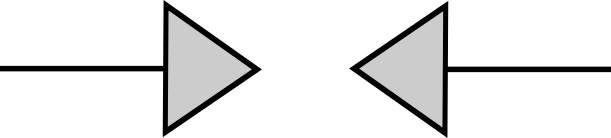
\includegraphics{figures/inkscape/path4585}
\end{center}


A $(p, q)$\textit{-tensor} is a linear function from $V^q$ to $V^p$. The space of such tensors $T^p_q (V)$ is isomorphic to $V^* \otimes ... \otimes V^* \otimes V \otimes ... \otimes V$ with $q$ copies of $V^*$ and $p$ copies of $V$. In tensor network diagrams, such a tensor is depicted as a box with $p$ wires going right and $q$ wires going left. As long as the endpoints are fixed, the shape of the wires does not matter.

\begin{center}
    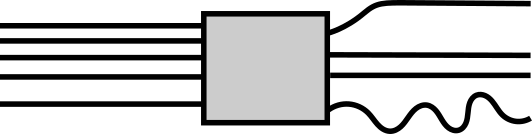
\includegraphics{figures/inkscape/tensor_box}
\end{center}

For example, a linear map $A: V \rightarrow V$ is depicted as a box with one wire on each side. The box itself can be annotated as well:

\begin{center}
    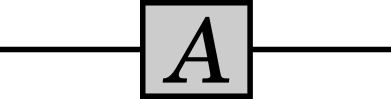
\includegraphics{figures/inkscape/box_a.png}
\end{center}

The tensor product of (arbitrary) tensors is depicted by drawing the two tensors one above the other:

\begin{center}
    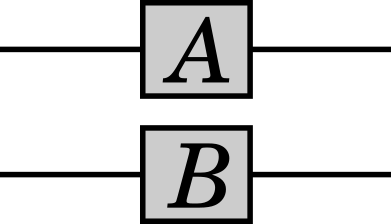
\includegraphics{figures/inkscape/tensor_product.png}
\end{center}


Since we work in $\mathbb{C}^d$ without any additional metric tensors, there are no extra tensors appearing when we raise or lower the indices of tensors. Pictorially, this means that we just bend the wires:

\begin{center}
    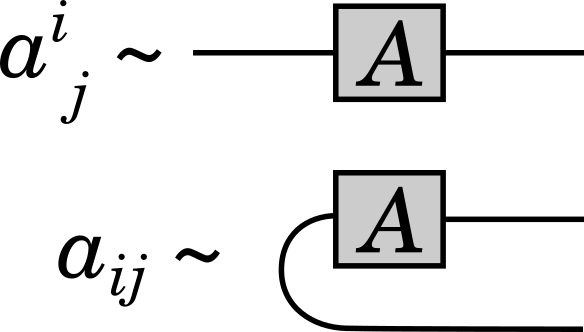
\includegraphics{figures/inkscape/bend_wires.png}
\end{center}

One must take care about the Hermitian conjugation operation (which is the combination of complex conjugation and transpose): we only denote it by explicitly marking tensors with the dagger sign ($\dagger$). The contraction of tensors is done by connecting the wires:

\begin{center}
    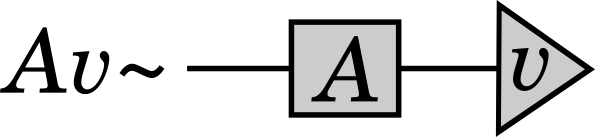
\includegraphics{figures/inkscape/contraction.png}
\end{center}

In particular, taking the trace of a matrix amounts to closing its wires into a loop:

\begin{center}
    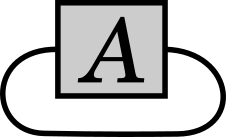
\includegraphics{figures/inkscape/trace.png}
\end{center}

It is also possible to consider linear functions over different vector spaces. For instance, when talking about mixed states, we can treat separately the internal degrees of freedom and the environment. In this case, one should just keep track of which wires belong to which space, either by subscripting them or by drawing them in different thickness, color, etc.

The convention on the direction of wires is completely arbitrary. The direction we choose here aligns with the mathematical notation of matrix multiplication, where the order they act on a vector is right to left. Quantum circuits are typically written in the opposite direction, so that the quantum gates are to be read left to right (the only exception we are aware of is \cite{kitaev_classical_2002}).

An interesting case of tensor networks are tensor network states, i.e.~quantum states that are best described as a contraction of certain tensors. For example, quantum circuits can be treated as such: wires are wires, and boxes are quantum gates. Suppose each qubit in a tensor network state is depicted by a distinct wire. Knowing the structure of the network, we can provide an upper bound to the amount of entanglement that will be found across any bipartition of the qubits. To do that, we split the network in two halves, so that each half only contains the outgoing wires of the respective partition of the qubit registry. There is no unique way to do this, and the bound will depend on the partition of the tensors. In any case, the halves will be connected by a number of wires. For the special case of quantum circuits we can assume that these are $w$ wires, each having the dimension equal to two. Schematically this situation in shown in Fig.~\ref{fig:cut}. If we now group the qubit spaces in bipartitions into two spaces, the tensor will essentially be a matrix with rank not exceeding $2^w$. The reduced density matrix of one of the halves is obtained from two copies of the tensor by contraction over a half of the open wires. The resulting tensor --- the density matrix --- also has the rank of $\leq 2^w$. It is then easy to see that the von Neumann entropy of this matrix is bound by $w$ ebits. Thus, the number of ebits in a bipartition is bounded by the number of cuts you need to make in order to split the tensor network diagram according to the bipartition.

\begin{figure}
    \centering
    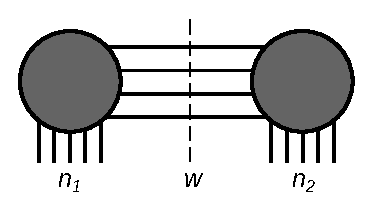
\includegraphics[width=0.5\linewidth]{figures/drawing_2.eps}
    \caption{A quantum circuit can be treated as a tensor network state with all bonds having dimension 2. If a bipartition cuts $w$ wires, the total bond dimension is at most $2^w$, while the cut separates at most $w$ ebits of entanglement. Reprinted from \cite{uvarov_machine_2020}.}
    \label{fig:cut}
\end{figure}

\section{Complexity-theoretical aspects of quantum computation}

% Goals of this section:
% Survey complexity-theoretical stuff about QCs
% Introduce 

How do quantum computers compare to classical computers? What is so different about them? To answer these questions, we must make a detour to the field of computational complexity. 

% A small detour into the field of quantum complexity is in order. To understand what kind of problems we want to solve, we should formalize the idea of a problem. 

% \begin{definition}
% An \textit{alphabet} is an arbitrary finite set $\Sigma$. The set of all possible finite-length words from this alphabet is denoted as $\Sigma^* := \bigcup_{n=0}^\infty \Sigma^n$.
% \end{definition}

% \begin{definition}
% A \textit{language} is a subset of $\Sigma^*$.
% \end{definition}

% ...
% It is important to distinguish a \textit{problem} and an \textit{instance} of a problem. 

\subsection{Classical complexity classes}


When we talk about problems that computers can or cannot solve, we mean the following. A \textit{problem} is a generic question of the kind ``Given $X$, find $Y$'', and an \textit{instance} of the problem is a specific value of $X$. When $Y$ is either yes or no, we call an instance a ``yes'' instance or a ``no'' instance, repsectively. Such yes or no problems are called \textit{decision problems}. 

Decision problems are grouped into complexity classes. Strictly speaking, the definitions of complexity classes rely on the notion of a Turing machine. However, for our purposes, we can equivalently define the most important complexity classes without having to introduce Turing machines. Complexity classes are usually defined by specifying how much time or space it takes to solve the problem as a function of the size of the input.

The complexity class $\mathbf{P}$ is defined as a class of problems that can be solved on a classical computer in polynomial time. This class includes many everyday problems solved by classical computers, such as sorting arrays of numbers, finding an element in an array, multiplying two matrices, etc. 

The class $\mathbf{NP}$ is defined as a class of decision problems where a solution to a ``yes'' instance of the problem can be efficiently verified with a classical computer. That is, if the answer to the question is ``yes'' and we are presented with some evidence of that (called \textit{witness}), we can quickly convince ourselves that the answer is indeed yes.


% The central construction of the theory of computation is the Turing machine. Informally, a deterministic Turing machine is a device that consists of an infinite tape and a moving head. The cells of a tape can have symbols written on them. The set of allowed symbols is called an \textit{alphabet}. Each time step, a head reads the symbol from the tape cell it stands on, changes its internal state, possibly rewrites the symbol in the cell, and moves one step left or right. Slightly more formally, the machine is described by the set of its possible states and a function that maps the tuple \textit{(state of the machine, symbol on the tape cell)} to the tuple \textit{(next state of the machine, new symbol on the cell, movement direction)}. One state of the machine is marked as the initial state, and at least one of the states is marked as terminal. This construction, from complexity-theoretical point of view, is an adequate description of any modern computer: If some algorithm can be run in polynomial time on any classical computer, it can also be run in polynomial time on a deterministic Turing machine.

% A significant change of the model is the \textit{nondeterministic Turing machine}. The main difference is that the function describing the machine can now take the state of the machine and return multiple different states. Informally, whenever there is a choice in the algorithm, a nondeterministic Turing machine can explore all options simultaneously. 

% These two constructions underlie the most famous open question of complexity theory, namely the $\mathbf{P} \overset{?}{=} \mathbf{NP}$ question. That is, does this nondeterministic Turing machine have greater computational power that a deterministic Turing machine? More concretely, $\mathbf{P}$ is defined as the class of problems that a deterministic Turing machine can solve in time that scales polynomially with the size of the input (for brevity, we will say ``this problem is solved in polynomial time''). The class $\mathbf{NP}$ is defined analogously for the nondeterministic Turing machine. 

% There are multiple reasons why the distinction of these classes is important. The class $\mathbf{P}$ is often considered to be class of decision problems that can be reasonably solved by a classical computer. However, many important problems actually lie in class $\mathbf{NP}$. The reason for that is that $\mathbf{NP}$ is also the class of problems where a solution to a ``yes'' instance of the problem can be efficiently verified with a classical computer. That is, if the answer to the question is ``yes'' and we are presented with some evidence of that (called \textit{witness}), we can quickly convince ourselves that the answer is indeed yes. 

\begin{example}[\textsc{Travelling salesperson}, decision version]
    Consider an edge-weighted, connected, undirected graph $G=(V, E)$ and a positive real number $L$. Decide if there exists a path that visits every vertex of the graph, such that the sum of the edges taken in the path is less than or equal to $L$. This is a problem in $\mathbf{NP}$ because the ``yes'' answer can be verified by providing such a path.
\end{example}

\begin{example}[\textsc{Circuit-SAT}]
    Given a Boolean circuit, decide if (``yes'') there is such an input that the first bit of the output evaluates to `1', or (``no'') for any input, the first bit evaluates to `0'. This problem is also in $\mathbf{NP}$ because the ``yes'' answer can be quickly verified by providing the correct input.
\end{example}

These two classes are the subject of the most famous open question of complexity theory, namely the $\mathbf{P} \overset{?}{=} \mathbf{NP}$ question. The distinction of these classes is important for the following reason. The class $\mathbf{P}$ is often considered to be the class of decision problems that can be reasonably solved by a classical computer. However, many important problems actually lie in class $\mathbf{NP}$.

The $\mathbf{NP}$ class is large and diverse, but there is a subclass of problems that stand out as the most difficult in this class. By relative difficulty we mean their \textit{Carp reducibility} to one another. Let $a$ is an instance of problem $A$, and let $f$ be a procedure that maps instances of problem $A$ to instances of problem $B$, taking ``yes'' instances to ``yes'' instances and ``no'' instances to ``no'' instances. In addition, let $f$ take polynomial time in the size of $a$. In this situation, we say that $A$ \textit{can be reduced to} $B$. 

If we now find an efficient procedure for solving $B$, this means that we can also efficiently solve $A$ by first mapping instances of $A$ to instances of $B$ and then solving the latter. That is why if $A$ is reduced to $B$, then $B$ is considered a more difficult problem.

A problem in $\mathbf{NP}$ such that all problems in $\mathbf{NP}$ can be reduced to it, is called an $\mathbf{NP}$-complete problem. The primary example of an $\mathbf{NP}$-complete problem is \textsc{Circuit-SAT}: the verifier of any problem in $\mathbf{NP}$ is a polynomial-time algorithm for a deterministic Turing machine, which can also be mapped to a polynomial-sized Boolean circuit. The completeness of \textsc{Circuit-SAT} is known as the Cook---Levin theorem \cite{cook_complexity_1971,levin_universal_1973}.

Finally, we should mention the complexity class $\mathbf{BPP}$. This class is defined as the class of problems that can be solved in polynomial time by a classical computer that also has access to a polynomial amount of random bits. Since such programs rely on randomness, we also demand that the probability of solving the problem wrong is bounded by $1/3$ regardless of the size of the input (this probability is actually arbitrary as long as it is fixed and strictly less than $1/2$). In this case, running the same algorithm $N$ times reduces the chance of error to $3^{-N}$.

The only known relation between these classes is that $\mathbf{P} \subseteq \mathbf{NP}$. It is generally believed that $\mathbf{P} \neq \mathbf{NP}$ and that $\mathbf{P} = \mathbf{BPP}$.

\subsection{Quantum complexity classes}

The first inquiries in quantum computation used the language of quantum Turing machines. In this model of computation, the elements of the tape are essentially qudits, the internal state of the machine is a quantum state, and the function that defines the next step is a unitary transformation \cite{bernstein_quantum_1997}.

% When the machine halts, we measure the state of the machine, which can in general be entangled. Analogously to the discussion above, we define the class $\mathbf{BQP}$ as the class of decision problems that can be solved by a quantum Turing machine in polynomial time, with error probability bounded by $1/3$. 

The quantum Turing machine model is equivalent to the model of quantum circuits, and thus we can define $\mathbf{BQP}$ as the class of problems that can be solved by polynomial-sized quantum circuits. The most famous example of a $\mathbf{BQP}$ problem is the problem of factoring integers into prime factors. The Shor's algorithm \cite{nielsen_quantum_2006} puts it into $\mathbf{BQP}$, while it is not known if it belongs to $\mathbf{P}$. It is not known how $\mathbf{BQP}$ compares to $\mathbf{P}$ or $\mathbf{NP}$. It is not difficult to show that $\mathbf{P} \in \mathbf{BQP}$, but the other direction is unknown. It is suspected that $\mathbf{BQP}$ is not included in $\mathbf{NP}$.
% , or even in the entire polynomial hierarchy, which is a sequence of nested complexity classes thought to be larger than $\mathbf{NP}$.

Just like $\mathbf{BQP}$ can be considered a quantum counterpart of $\mathbf{P}$ (or more precisely, $\mathbf{BPP}$), the class $\mathbf{NP}$ has a quantum counterpart, too. This class is called $\mathbf{QMA}$ and contains problems that can be efficiently verified with a quantum computer. The name of the class $\mathbf{QMA}$ is an acronym for ``Quantum Merlin--Arthur''. This name comes from a hypothetical scenario featuring Arthur, king of the Britons, and Merlin, a mighty wizard and advisor to Arthur. Merlin can solve any problem, but Arthur doesn't trust him too much and wants to be able to verify Merlin's suggestions. To convince Arthur that the ``yes'' instance is indeed a ``yes'' instance, Merlin can provide a polynomial-sized quantum state. More precisely, for ``yes'' instances, Arthur should be able to correctly verify it with probability above $2/3$, while for the ``no'' instance, Merlin should not be able to fool Arthur into believing that it's a ``yes'' instance with probability above $1/3$. Again, here the probabilities are with respect to Arthur's source of randomness, so by running his algorithm more than once, he can achive any desired level of confidence.

In fact, all complexity classes above (and some more) can be specified in terms of what Arthur can do and what Merlin can provide him as proof of his words. The resources of Arthur and Merlin are summarized in Table \ref{tab:complexity_classes}.

\begin{table}
    \centering
    \begin{tabularx}{\textwidth}{|lXl|}
        \hline
        \textbf{Class} & \textbf{Arthur has a...} & \textbf{Merlin can provide...} \\
        \hline
        $\mathbf{P}$ & classical computer & nothing \\
        $\mathbf{BPP}$ & classical computer and a source of randomness & nothing\\
        $\mathbf{NP}$ & classical computer & a polynomially-long string \\
        $\mathbf{MA}$ & classical computer and a source of randomness &  a polynomially-long string \\
        $\mathbf{BQP}$ & quantum computer & nothing \\
        $\mathbf{QMA}$ & quantum computer & a quantum state in $poly(n)$ qubits\\
        $\mathbf{QCMA}$ & quantum computer & a polynomially-long string\\
        \hline
   \end{tabularx}
   \caption{\label{tab:complexity_classes}Complexity classes described as an interaction between Arthur and Merlin.}
\end{table}

A canonical $\mathbf{QMA}$-complete problem is \textsc{Quantum circuit-SAT}: given a quantum circuit, decide if there is any input quantum state such that the first qubit of the output is measured in the state $\ket{1}$. This problem is $\mathbf{QMA}$-complete almost by definition: it is in $\mathbf{QMA}$ because the input state is a witness, and it is complete for $\mathbf{QMA}$ because for any problem in $\mathbf{QMA}$, you can construct a verifier circuit, and now if you ask if this verifier circuit ever returns a $\ket{1}$, you obtain an instance of \textsc{Quantum circuit-SAT}.

An ingenious construction due to Kitaev and coworkers \cite{kitaev_classical_2002} proves that the problem of finding a low-energy state of a local Hamiltonian is also $\mathbf{QMA}$-complete.

\begin{definition}[$k$-\textsc{Local Hamiltonian}]
    Given: $(H, a, b)$, where:
    \begin{enumerate}
        \item $H = \sum_i H_i$ is a Hamiltonian acting on a product of $n$ subsystems. The terms $H_i$ have operator norm bounded by a constant and support bounded by $k \in \mathbb{N}$. For each subsystem, the number of terms acting nontrivially on that subsystem is also bounded by a constant in $n$.
        \item $a, b \in \mathbb{R}$, such that $a < b$ and $b - a \geq O(1/ poly(n))$.
    \end{enumerate}
    Decide if there is a state $\ket{\psi}$ such that $\bra{\psi}H\ket{\psi} \leq a$ or if all states have energy above $\bra{\psi}H\ket{\psi} \geq b$, promised that either is the case.
\end{definition}

% Notice that we introduced promise that the ground state energy of the Hamiltonian does not belong to the gap $(a, b)$. The role of this gap is as follows\dots

This problem was first proven to be $\mathbf{QMA}$-complete for $k \geq 5$ \cite{kitaev_classical_2002}. Then, it was gradually improved to lower values of $k$ \cite{kempe_3-local_2003}, until it was ultimately proven complete even for $k = 2$ \cite{kempe_complexity_2006}. Note that for $k = 1$ this problem is in $\mathbf{P}$: each term can just be minimized independently.

In the following chapters, we will mostly deal with instances of \textsc{Local Hamiltonian}. 
A plausible complexity-theoretic assumption is that $\mathbf{BQP} \neq \mathbf{QMA}$, which means we may never be able to solve this problem efficiently, even with scalable, fault-tolerant quantum computers. 
However, not all is lost. In classical computing, the fact that a problem is $\mathbf{NP}$-complete only implies that the worst instances are hard to solve, while many real instances turn out to have good approximate solutions. Arguably, the entire effort of variational quantum algorithms is devoted to finding good heuristic algorithms for $\mathbf{QMA}$-complete problems.







